
% \section{Decay data} \label{sec:fe_data}
% % 
% % % \begin{longtable}{|c|c|c|c|c|} 
% % % \caption{My caption}
% % % \label{tab:dummy}
% % % % \begin{tabular}{|c|c|c|c|c|}
% % %    \hline
% % %  
% % % \end{longtable}
% % Table of decay data  for observed gamma-rays. 
% The   lifetimes and gamma-ray branching ratios  listed in these tables were used for all calculations of measured cross sections reported in this work, and have been taken from the most recent edition of  Nuclear Data Sheets for each  mass chain 
% % \cite{Basunia2015,Firestone2007,Wang2017,Dong2015,Dong2014,JUNDE2008787,Junde2011,Bhat1998,Nesaraja2010,BAGLIN2002,Browne2013,Zuber20151,NICHOLS2012973,Singh2007,Browne2010,Tuli2003,McCutchan2015,Singh2014,NEGRET20151,Johnson2015,McCutchan2014,Singh2013,Browne1997,Baglin2013,Baglin2012,Baglin2011}. 
% 
% 
% 
% % Preview source code for paragraph 0
% 
% \begin{table}[ht]
% \centering
% \caption{Decay data for gamma-rays observed in \ce{^{nat}Ti}(p,x) and \ce{^{nat}Cu}(p,x).}
% \label{tab:fe_nudat_table_monitors}
% \small
% % \resizebox{\textheight}{!}{%
% % Disable adjustbox for journal submission
% % \begin{adjustbox}{totalheight=\textheight-2\baselineskip}
% \begin{tabular}{@{}llll@{}}
% \toprule
% % \begin{tabular}{|c|c|c|c|}
% % \hline 
% Nuclide & Half-life & E$_\gamma$ (keV) & I$_\gamma$ (\%)\\
% \midrule
% \ce{^{22}Na} & 2.6018(22) y & 1274.537 & 99.940(14)\\
%  
% % \ce{^{24}Na} & 14.997(12) h & 1368.626 & 99.9936(15)\\
% %  
% % \ce{^{51}Cr} & 27.704(3) d & 320.0824 & 9.910(10)\\
% %  
% % \ce{^{52m}Mn} & 21.1(2) m & 1434.0600 & 98.2(5)\\
% %  
% % \ce{^{52}Mn} & 5.591(3) d & 744.233 & 90.0(12)\\
% %  
% %  & 5.591(3) d & 935.544 & 94.5(13)\\
% %  
% %  & 5.591(3) d & 1246.278 & 4.21(7)\\
% %  
% %  & 5.591(3) d & 1434.092 & 100.0(14)\\
% %  
% % \ce{^{54}Mn} & 312.20(20) & 834.848 & 99.9760(10)\\
% %  
% % \ce{^{55}Co} & 17.53(3) h & 477.2 & 20.2(17)\\
% %  
% %  & 17.53(3) h & 931.1 & 75.0(35)\\
% %  
% %  & 17.53(3) h & 1316.6 & 7.1(3)\\
% %  
% %  & 17.53(3) h & 1408.5 & 16.9(8)\\
% %  
% % \ce{^{56}Ni} & 6.075(10) d & 158.38 & 98.8(10)\\
% %  
% %  & 6.075(10) d & 269.50 & 36.5(8)\\
% %  
% %  & 6.075(10) d & 480.44 & 36.5(8)\\
% %  
% %  & 6.075(10) d & 749.95 & 49.5(12)\\
% %  
% %  & 6.075(10) d & 811.85 & 86.0(9)\\
% %  
% %  & 6.075(10) d & 1561.80 & 14.0(6)\\
% %  
% % \ce{^{56}Co} & 77.236(26) d & 846.770 & 99.9399(2)\\
% %  
% % %  & 77.236(26) d & 977.372 & 1.421(6)\\
% %  
% %  & 77.236(26) d & 1037.843 & 14.05(4)\\
% %  
% %  & 77.236(26) d & 1238.288 & 66.46(12)\\
% %  
% %  & 77.236(26) d & 1360.212 & 4.283(12)\\
% %  
% %  & 77.236(26) d & 1771.357 & 15.41(6)\\
% %  
% % \ce{^{57}Ni} & 35.60(6) h & 127.164 & 16.7(5)\\
% %  
% %  & 35.60(6) h & 1377.63 & 81.7(24)\\
% %  
% %  & 35.60(6) h & 1757.55 & 5.75(20)\\
% %  
% %  & 35.60(6) h & 1919.52 & 12.3(4)\\
% %  
% % \ce{^{57}Co} & 271.74(6) d & 122.06065 & 85.60(17)\\
% %  
% %  & 271.74(6) d & 136.47356 & 10.68(8)\\
% %  
% % \ce{^{58}Co} & 70.86(6) d & 810.7593 & 99.450(10)\\
% %  
% %  & 70.86(6) d & 863.951 & 0.686(10)\\
% %  
% % %  & 70.86(6) d & 1674.725 & 0.517(10)\\
% %  
% % \ce{^{59}Fe} & 44.495(9) d & 1099.245 & 56.5(18)\\
% %  
% %  & 44.495(9) d & 1291.590 & 43.2(14)\\
% %  
% % \ce{^{60}Co} & 5.2714(5) y & 1173.228 & 99.85(3)\\
% %  
% %  & 5.2714(5) y & 1332.492 & 99.9826(6)\\
% %  
% % \ce{^{61}Cu} & 3.339(8) h & 282.956 & 12.2(2.2)\\
% %  
% %  & 3.339(8) h & 373.050 & 2.1(4)\\
% %  
% % %  & 3.339(8) h & 588.605 & 1.17(21)\\
% %  
% %  & 3.339(8) h & 656.008 & 10.8(20)\\
% %  
% %  & 3.339(8) h & 1185.234 & 3.7(7)\\
% %  
% % \ce{^{62}Zn} & 9.193(15) h & 243.36 & 2.52(23)\\
% %  
% %  & 9.193(15) h & 246.95 & 1.90(18)\\
% %  
% %  & 9.193(15) h & 260.43 & 1.35(13)\\
% %  
% % %  & 9.193(15) h & 304.88 & 0.29(3)\\
% %  
% % %  & 9.193(15) h & 349.60 & 0.45(4)\\
% %  
% %  & 9.193(15) h & 394.03 & 2.24(17)\\
% %  
% %  & 9.193(15) h & 548.35 & 15.3(14)\\
% %  
% %  & 9.193(15) h & 596.56 & 26.0(20)\\
% %  
% % %  & 9.193(15) h & 637.41 & 0.25(3)\\
% %  
% % \ce{^{64}Cu} & 12.701(2) h & 1345.77 & 0.475(11)\\
% %  
% % \ce{^{65}Zn} & 243.93(9) d & 1115.539 & 50.04(10)\\
% \bottomrule
% \end{tabular}
% % }
% % \end{adjustbox}
% \end{table}
% 
% 
% 
% \begin{table}[ht]
% \centering
% \caption{Decay data for gamma-rays observed in \ce{^{nat}Fe}(p,x).}
% \label{tab:fe_nudat_table_nb}
% \small
% % \resizebox{\textheight}{!}{%
% % Disable adjustbox for journal submission
% % \begin{adjustbox}{totalheight=\textheight-2\baselineskip}
% \begin{tabular}{@{}llll@{}}
% \toprule
% % \begin{tabular}{|c|c|c|c|}
% % \hline 
% Nuclide & Half-life & E$_\gamma$ (keV) & I$_\gamma$ (\%)\\
% \midrule
% \ce{^{82m}Rb} & 6.472(6) h & 554.35 & 62.4(9)\\
%  
%  & 6.472(6) h & 619.11 & 37.98(9)\\
%  
% %  & 6.472(6) h & 698.37 & 26.3(7)\\
%  
% %  & 6.472(6) h & 776.52 & 84.39(21)\\
% %  
% %  & 6.472(6) h & 1044.08 & 32.07(8)\\
% %  
% % %  & 6.472(6) h & 1317.43 & 23.7(6)\\
% %  
% % \ce{^{83}Sr} & 32.41(3) h & 418.37 & 4.2(3)\\
% %  
% %  & 32.41(3) h & 762.65 & 26.7(22)\\
% %  
% % \ce{^{85m}Y} & 4.86(13) h & 231.7 & 22.8(22)\\
% %  
% % \ce{^{85}Y} & 2.68(5) h & 231.65 & 84(9)\\
% %  
% %  & 2.68(5) h & 913.89 & 9.0(9)\\
% %  
% % \ce{^{86}Zr} & 16.5(1) h & 242.8 & 95.84(2)\\
% %  
% %  & 16.5(1) h & 612.0 & 5.8(3)\\
% %  
% % % \ce{^{86}Y} & 14.74(2) h & 187.87 & 1.26(4)\\
% % \ce{^{86}Y}  & 14.74(2) h & 443.13 & 16.9(5)\\
% % 
% %  
% % %  & 14.74(2) h & 190.80 & 1.01(3)\\
% %  
% % %  & 14.74(2) h & 307.00 & 3.47(8)\\
% %  
% % %  & 14.74(2) h & 443.13 & 16.9(5)\\
% %  
% % %  & 14.74(2) h & 580.57 & 4.78(14)\\
% %  
% % %  & 14.74(2) h & 608.29 & 2.01(15)\\
% %  
% %  & 14.74(2) h & 627.72 & 32.6(1)\\
% %  
% % %  & 14.74(2) h & 703.33 & 15.4(4)\\
% %  
% % %  & 14.74(2) h & 709.90 & 2.62(8)\\
% %  
% % %  & 14.74(2) h & 767.63 & 2.4(3)\\
% %  
% % %  & 14.74(2) h & 835.67 & 4.4(6)\\
% %  
% % %  & 14.74(2) h & 1024.04 & 3.79(17)\\
% %  
% %  & 14.74(2) h & 1076.63 & 82.5(4)\\
% %  
% %  & 14.74(2) h & 1153.05 & 30.5(9)\\
% %  
% % %  & 14.74(2) h & 1163.03 & 1.18(4)\\
% % %  
% % %  & 14.74(2) h & 1253.11 & 1.53(5)\\
% %  
% % %  & 14.74(2) h & 1349.15 & 2.95(9)\\
% %  
% %  & 14.74(2) h & 1854.38 & 17.2(5)\\
% %  
% %  & 14.74(2) h & 1920.72 & 20.8(7)\\
% %  
% % \ce{^{87}Zr} & 1.68(1) h & 380.79 & 62.79(10)\\
% %  
% %  & 1.68(1) h & 1227.0 & 2.80(4)\\
% %  
% % \ce{^{87m}Y} & 13.37(1) h & 380.79 & 78.05(8)\\
% %  
% % \ce{^{87}Y} & 79.8(3) h & 388.5276 & 82.2(7)\\
% %  
% %  & 79.8(3) h & 484.805 & 89.8(9)\\
% %  
% % \ce{^{88}Zr} & 83.4(3) d & 392.87 & 97.29(14)\\
% %  
% % \ce{^{88}Y} & 106.627(21) d & 898.042 & 93.7(3)\\
% %  
% %  & 106.627(21) d & 1836.063 & 99.2(3)\\
% %  
% % \ce{^{89m}Nb} & 66(2) m & 588.0 & 95.57(13)\\
% %  
% % \ce{^{89}Nb} & 2.03(7) h & 1511.4 & 1.9(4)\\
% %  
% %  & 2.03(7) h & 1627.2 & 3.5(7)\\
% %  
% %  & 2.03(7) h & 1833.4 & 3.3(7)\\
% %  
% % \ce{^{89}Zr} & 78.41(12) h & 909.15 & 99.04(3)\\
% %  
% %  & 78.41(12) h & 1713.0 & 0.745(13)\\
% %  
% % %  & 78.41(12) h & 1744.5 & 0.123(4)\\
% %  
% % \ce{^{90}Mo} & 5.56(9) h & 122.370 & 64(3)\\
% %  
% %  & 5.56(9) h & 162.93 & 6.0(6)\\
% %  
% %  & 5.56(9) h & 203.13 & 6.4(6)\\
% %  
% %  & 5.56(9) h & 257.34 & 78(4)\\
% %  
% %  & 5.56(9) h & 323.20 & 6.3(6)\\
% %  
% %  & 5.56(9) h & 472.2 & 1.42(16)\\
% %  
% %  & 5.56(9) h & 941.5 & 5.5(7)\\
% %  
% % \ce{^{90}Nb} & 14.6(5) h & 132.716 & 4.13(4)\\
% %  
% %  & 14.6(5) h & 141.178 & 66.8(7)\\
% %  
% % %  & 14.6(5) h & 890.64 & 1.80(4)\\
% %  
% %  & 14.6(5) h & 1611.76 & 2.38(7)\\
% %  
% % %  & 14.6(5) h & 1913.194 & 1.280(17)\\
% %  
% % \ce{^{91m}Nb} & 60.86(22) d & 104.62 & 0.574(1)\\
% %  
% %  & 60.86(22) d & 1204.67 & 2.0(3)\\
% %  
% % \ce{^{92m}Nb} & 10.15(2) d & 912.6 & 1.78(10)\\
% %  
% %  & 10.15(2) d & 934.44 & 99.15(4)\\
% %  
% % \ce{^{93m}Mo} & 6.85(7) d & 263.049 & 57.4(11)\\
% %  
% %  & 6.85(7) d & 684.693 & 99.9(8)\\
% %  
% %  & 6.85(7) d & 1477.138 & 99.1(11)\\
% \bottomrule
% \end{tabular}
% % }
% % \end{adjustbox}
% \end{table}
% 

% 
% 
\section{Measured excitation functions} \label{sec:fe_xs_figures}

Figures of the cross sections measured in this work are presented here, in comparison with literature data
\cite{Al-Abyad2009,A2006,Aleksandrov1987,barchuk1987excitation,Barrandon1975,Belhout2007,Brodzinski1971,Brodzinski1971a,daum1997investigation,Ditroi2005,Fink1990,Garrido2016,Graves2016,Greenwood1984,Grutter1982,Jung1987,Khandaker2009,Kim2014,Kopecky1993,Lagunas-Solar1979a,levkovski1991cross,MICHEL1997153,MICHEL1979a,Michel1980,Michel1978,Michel1985,Mills1992,Neumann1999a,Schoen1979a,Shahid2015,Sudar1994,Takacs1994a,Voyles2018a,PhysRev.162.1055,YashimaH2003,Zarie2006a,zhao1993measurement}.

% \comment{Add in CoH model output from Toshihiko to all plots}





% Prevent ''overfull hbox'' warnings for < 5pt overflow 
% \hfuzz=10pt 

\begin{figure*}
    \sloppy
    \centering
    \subfloat{
        \centering
%         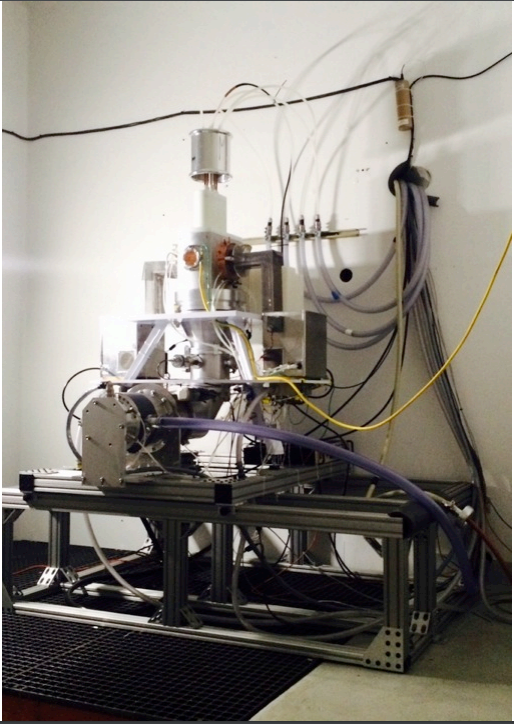
\includegraphics[width=\columnwidth]{./figures/Capture.PNG}
        \subfigimg[width=0.496\textwidth]{}{./figures/48Cr.pdf}{50}
%         \caption{ Decay curve for the isomeric transition of \ce{^{115m}In}.}
%         \refstepcounter{subfigure}
%          \label{fig:51Cr}%
%         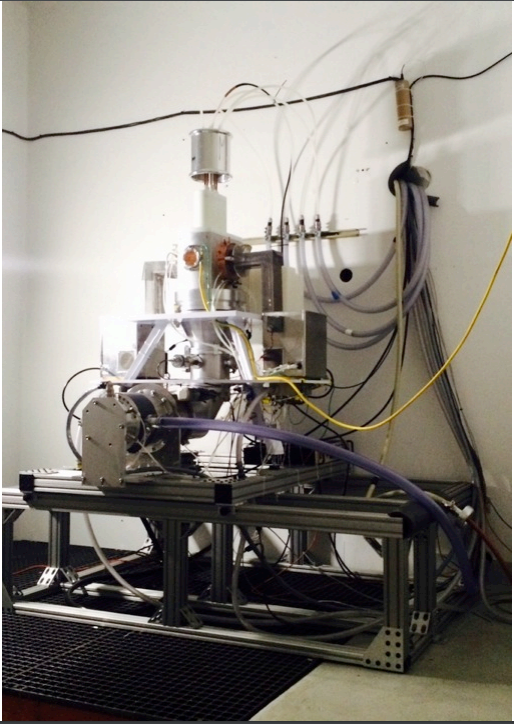
\includegraphics[width=\columnwidth]{./figures/Capture.PNG}
%         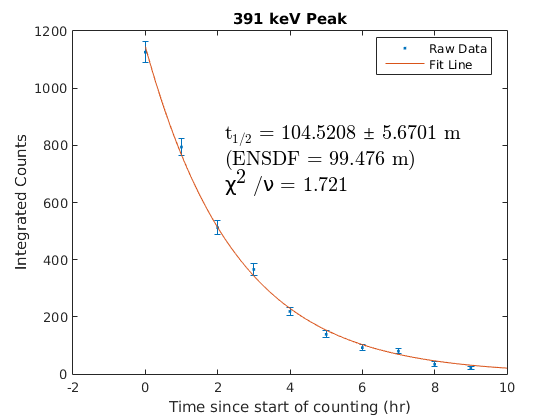
\includegraphics[scale=0.6]{./figures/391keV_curve2.png}
        \subfigimg[width=0.496\textwidth]{}{./figures/48V_ind.pdf}{50}
%         \caption{ Decay curve for the isomeric transition of \ce{^{113m}In}.}
%         \refstepcounter{subfigure}
%          \label{fig:52Mn}
   \hspace{-10pt}}%
    \\
    \subfloat{
        \centering
%         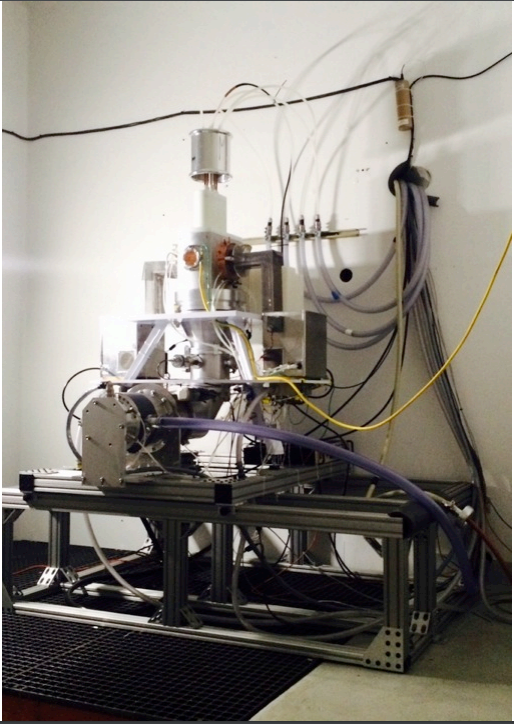
\includegraphics[width=\columnwidth]{./figures/Capture.PNG}
        \subfigimg[width=0.496\textwidth]{}{./figures/48V_cum.pdf}{50}
%         \caption{ Decay curve for the isomeric transition of \ce{^{115m}In}.}
%         \refstepcounter{subfigure}
%          \label{fig:52gMn}%
%         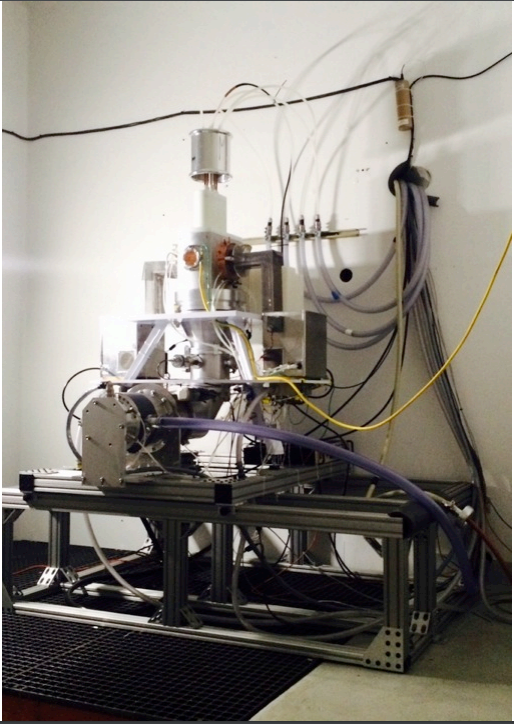
\includegraphics[width=\columnwidth]{./figures/Capture.PNG}
%         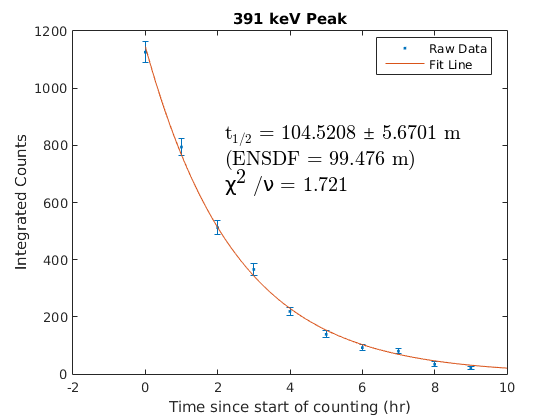
\includegraphics[scale=0.6]{./figures/391keV_curve2.png}
        \subfigimg[width=0.496\textwidth]{}{./figures/49Cr.pdf}{50}
%         \caption{ Decay curve for the isomeric transition of \ce{^{113m}In}.}
%         \refstepcounter{subfigure}
%          \label{fig:52mMn}
   \hspace{-10pt}}%
    \\
    \subfloat{
        \centering
%         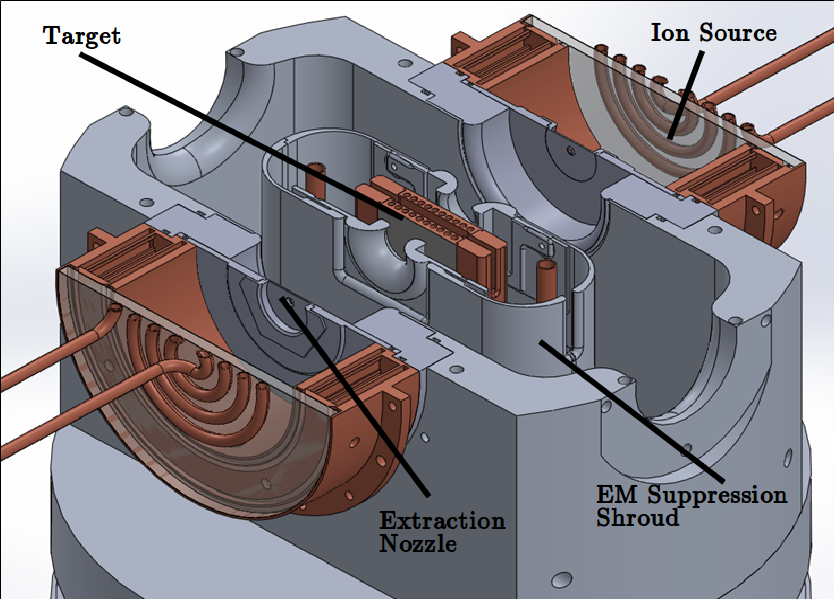
\includegraphics[width=\textwidth]{./figures/target2.png}
        \subfigimg[width=0.496\textwidth]{}{./figures/51Cr_ind.pdf}{50}
%         \caption{Decay curve for the $\beta^-$ decay of \ce{^{116}In}.}
        %         \refstepcounter{subfigure}
%          \label{fig:54Mn}
%
%         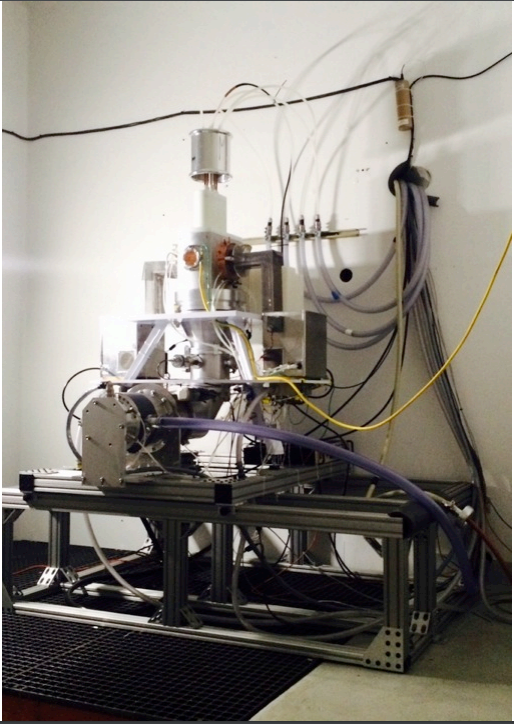
\includegraphics[width=\columnwidth]{./figures/Capture.PNG}
        \subfigimg[width=0.496\textwidth]{}{./figures/51Cr_cum.pdf}{50}
%         \caption{ Decay curve for the $\beta^+$ decay of \ce{^{64}Cu}.}
%         \refstepcounter{subfigure} 
%         \label{fig:55Co}
   \hspace{-10pt}}%
%     \caption{Decay curves used to verify photopeak transition assignment. (a) Decay curve for the isomeric transition of \ce{^{115m}In}, (b) decay curve for the isomeric transition of \ce{^{113m}In}, (c) decay curve for the $\beta^-$ decay of \ce{^{116}In}, and (d) decay curve for the $\beta^+$ decay of \ce{^{64}Cu}.}
%      \phantomcaption{}\label{fig:xs_curves_p1}
\end{figure*}




\begin{figure*}
    \centering
    \subfloat{
        \centering
%         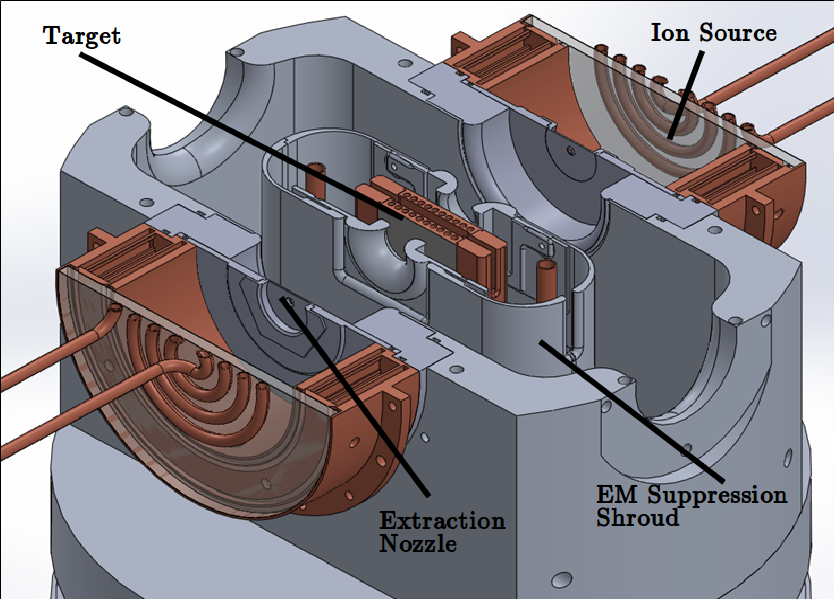
\includegraphics[width=\textwidth]{./figures/target2.png}
        \subfigimg[width=0.496\textwidth]{}{./figures/52gMn.pdf}{50}
%         \caption{Decay curve for the $\beta^-$ decay of \ce{^{116}In}.}
        %         \refstepcounter{subfigure}
%          \label{fig:56Ni}
%
%         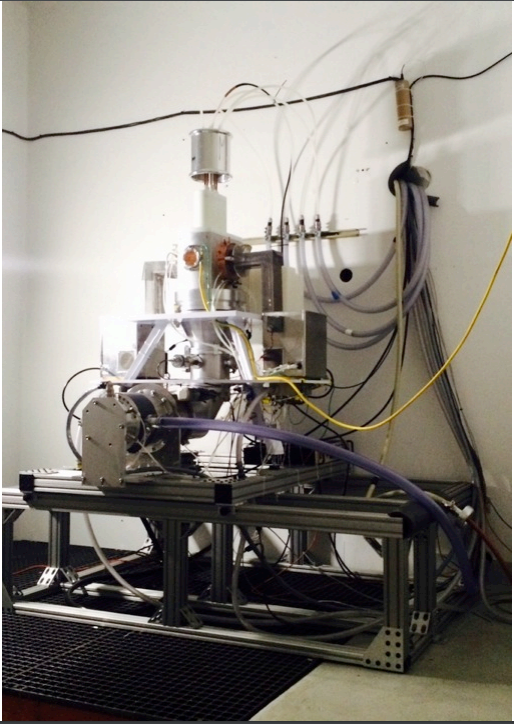
\includegraphics[width=\columnwidth]{./figures/Capture.PNG}
        \subfigimg[width=0.496\textwidth]{}{./figures/52Fe.pdf}{50}
%         \caption{ Decay curve for the $\beta^+$ decay of \ce{^{64}Cu}.}
%         \refstepcounter{subfigure}
%         \label{fig:57Co}
   \hspace{-10pt}}%
    \\
    \subfloat{
        \centering
%         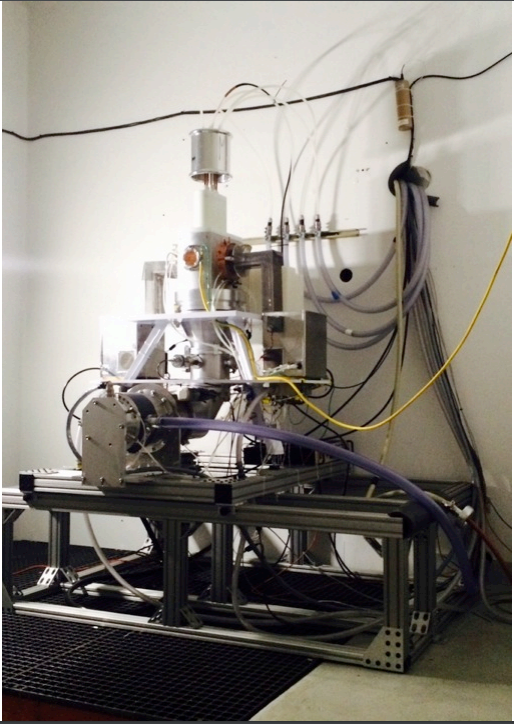
\includegraphics[width=\columnwidth]{./figures/Capture.PNG}
        \subfigimg[width=0.496\textwidth]{}{./figures/54Mn.pdf}{50}
%         \caption{ Decay curve for the isomeric transition of \ce{^{115m}In}.}
%         \refstepcounter{subfigure}
%          \label{fig:57Ni}%
%         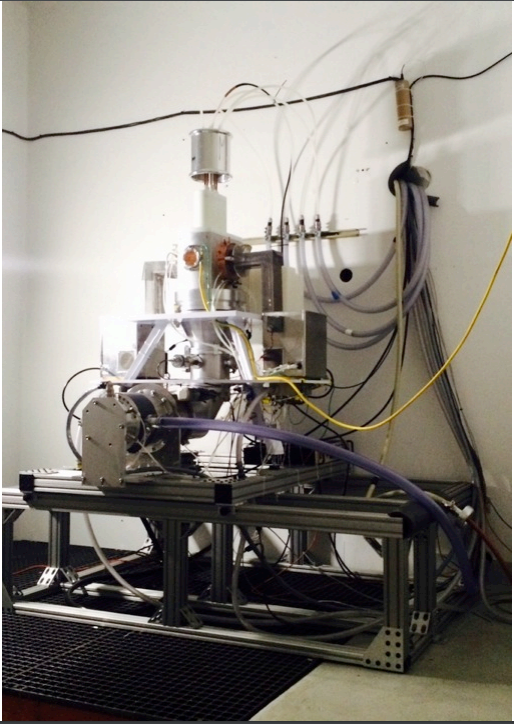
\includegraphics[width=\columnwidth]{./figures/Capture.PNG}
%         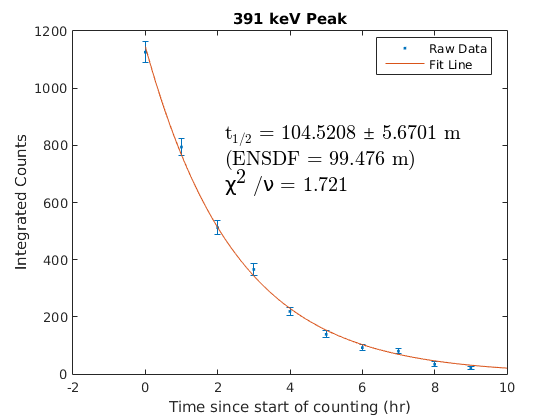
\includegraphics[scale=0.6]{./figures/391keV_curve2.png}
        \subfigimg[width=0.496\textwidth]{}{./figures/55Co.pdf}{50}
%         \caption{ Decay curve for the isomeric transition of \ce{^{113m}In}.}
%         \refstepcounter{subfigure}
%          \label{fig:58Co}
   \hspace{-10pt}}%
    \\
    \subfloat{
        \centering
%         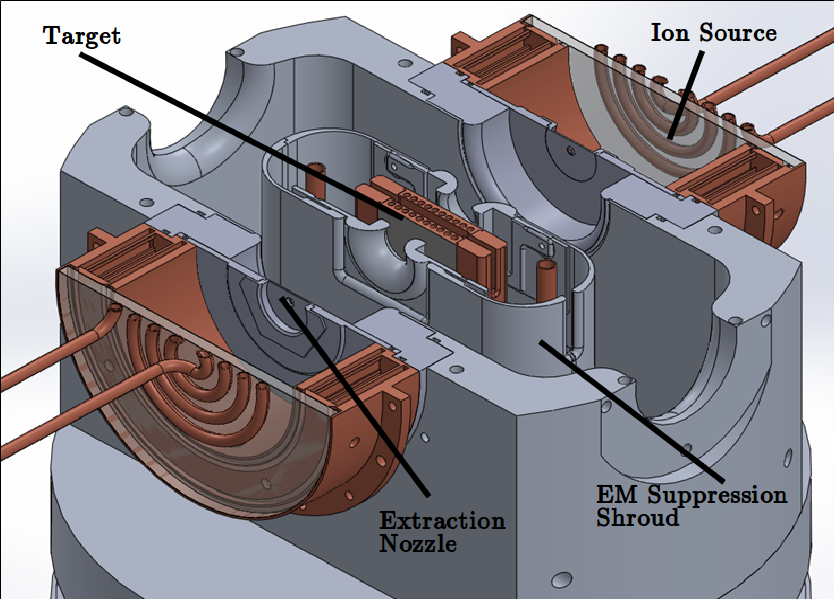
\includegraphics[width=\textwidth]{./figures/target2.png}
        \subfigimg[width=0.496\textwidth]{}{./figures/56Mn.pdf}{50}
%         \caption{Decay curve for the $\beta^-$ decay of \ce{^{116}In}.}
        %         \refstepcounter{subfigure}
%          \label{fig:58gCo}
%
%         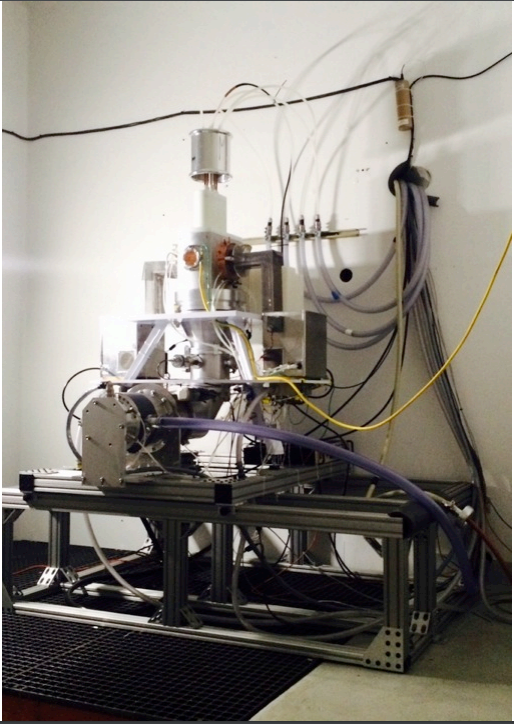
\includegraphics[width=\columnwidth]{./figures/Capture.PNG}
        \subfigimg[width=0.496\textwidth]{}{./figures/56Co.pdf}{50}
%         \caption{ Decay curve for the $\beta^+$ decay of \ce{^{64}Cu}.}
%         \refstepcounter{subfigure}
%         \label{fig:58mCo}
   \hspace{-10pt}}%
%     \caption{Decay curves used to verify photopeak transition assignment. (a) Decay curve for the isomeric transition of \ce{^{115m}In}, (b) decay curve for the isomeric transition of \ce{^{113m}In}, (c) decay curve for the $\beta^-$ decay of \ce{^{116}In}, and (d) decay curve for the $\beta^+$ decay of \ce{^{64}Cu}.}
%      \phantomcaption{}\label{fig:xs_curves_p2}
\end{figure*}



\begin{figure*}
    \centering
    \subfloat{
        \centering
%         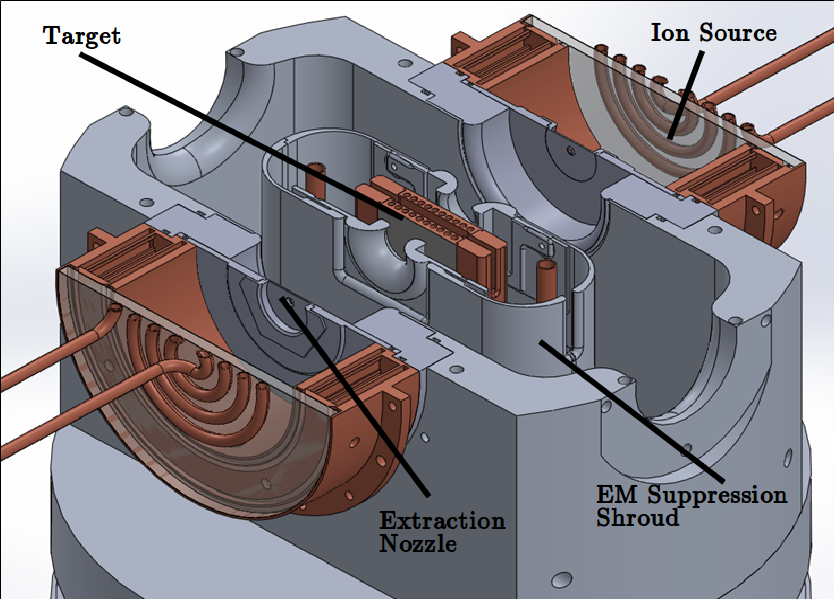
\includegraphics[width=\textwidth]{./figures/target2.png}
        \subfigimg[width=0.496\textwidth]{}{./figures/57Co.pdf}{50}
%         \caption{Decay curve for the $\beta^-$ decay of \ce{^{116}In}.}
        %         \refstepcounter{subfigure}
%          \label{fig:59Fe}
%
%         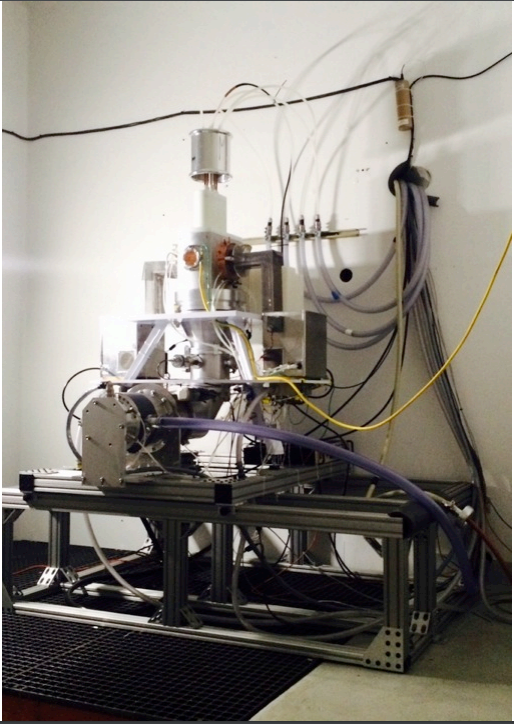
\includegraphics[width=\columnwidth]{./figures/Capture.PNG}
        \subfigimg[width=0.496\textwidth]{}{./figures/58mCo.pdf}{50}
%         \caption{ Decay curve for the $\beta^+$ decay of \ce{^{64}Cu}.}
%         \refstepcounter{subfigure} 
%         \label{fig:60Co}
   \hspace{-10pt}}%
    \\
    \subfloat{
        \centering
%         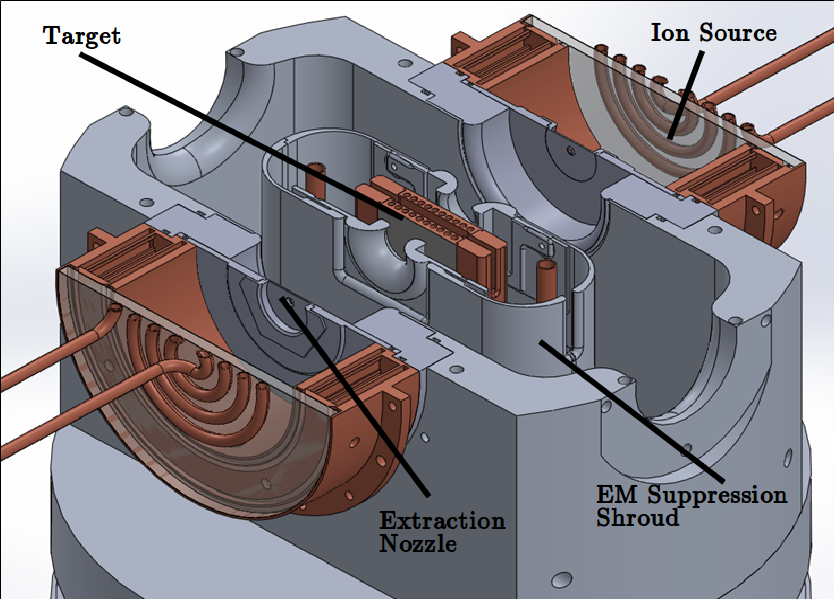
\includegraphics[width=\textwidth]{./figures/target2.png}
        \subfigimg[width=0.496\textwidth]{}{./figures/58gCo.pdf}{50}
%         \caption{Decay curve for the $\beta^-$ decay of \ce{^{116}In}.}
        %         \refstepcounter{subfigure}
%          \label{fig:61Cu}
%
%         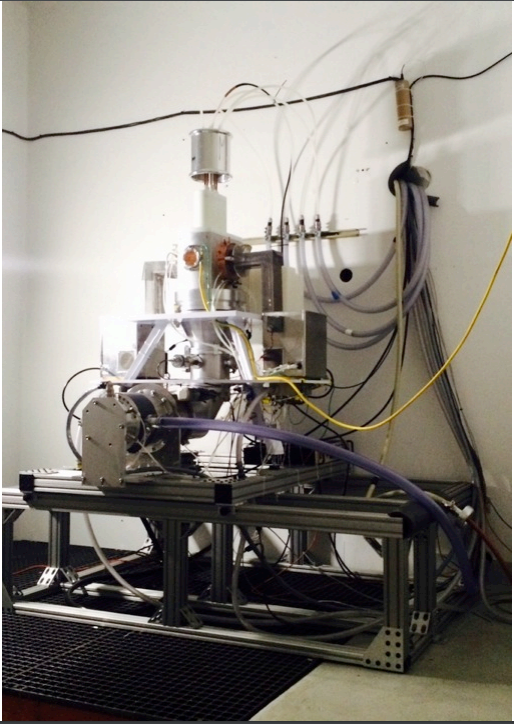
\includegraphics[width=\columnwidth]{./figures/Capture.PNG}
        \subfigimg[width=0.496\textwidth]{}{./figures/58Co.pdf}{50}
%         \caption{ Decay curve for the $\beta^+$ decay of \ce{^{64}Cu}.}
%         \refstepcounter{subfigure}
%         \label{fig:64Cu}
   \hspace{-10pt}}%
    \\
    \subfloat{
        \centering
%         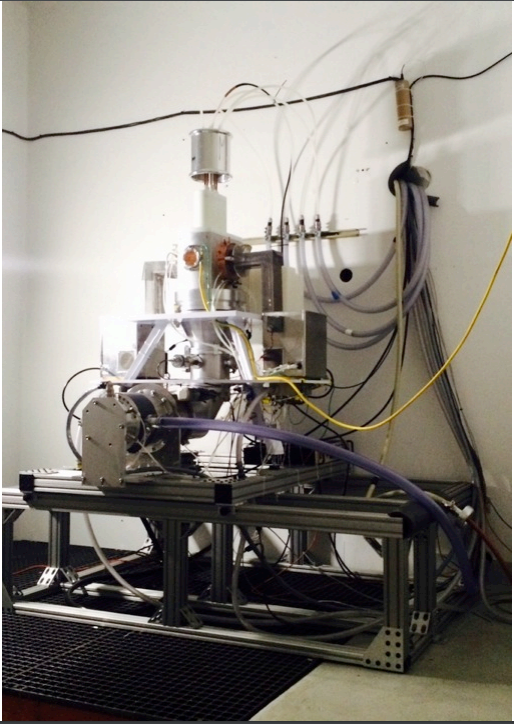
\includegraphics[width=\columnwidth]{./figures/Capture.PNG}
        \subfigimg[width=0.496\textwidth]{}{./figures/54MnCu.pdf}{50}
%         \caption{ Decay curve for the isomeric transition of \ce{^{115m}In}.}
%         \refstepcounter{subfigure}
%          \label{fig:82mRb}%
%         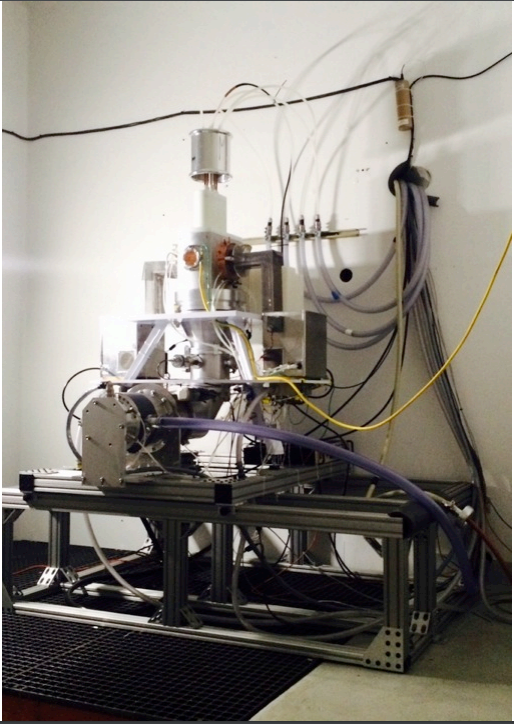
\includegraphics[width=\columnwidth]{./figures/Capture.PNG}
%         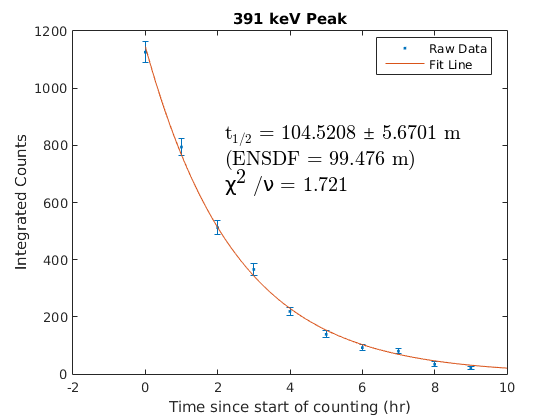
\includegraphics[scale=0.6]{./figures/391keV_curve2.png}
        \subfigimg[width=0.496\textwidth]{}{./figures/57Ni.pdf}{50}
%         \caption{ Decay curve for the isomeric transition of \ce{^{113m}In}.}
%         \refstepcounter{subfigure}
%          \label{fig:83Sr}
   \hspace{-10pt}}%
%     \caption{Decay curves used to verify photopeak transition assignment. (a) Decay curve for the isomeric transition of \ce{^{115m}In}, (b) decay curve for the isomeric transition of \ce{^{113m}In}, (c) decay curve for the $\beta^-$ decay of \ce{^{116}In}, and (d) decay curve for the $\beta^+$ decay of \ce{^{64}Cu}.}
%      \phantomcaption{}\label{fig:xs_curves_p3}
\end{figure*}



\begin{figure*}
    \centering
    \subfloat{
        \centering
%         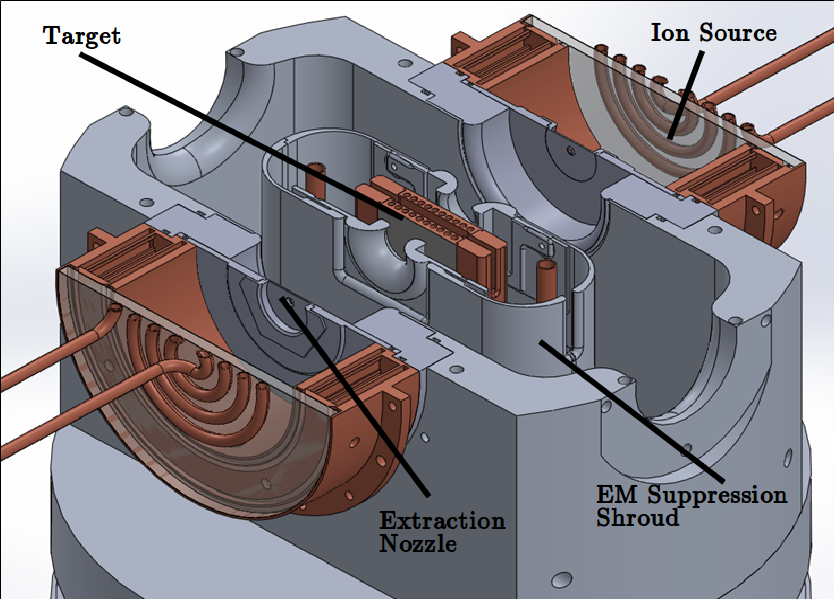
\includegraphics[width=\textwidth]{./figures/target2.png}
        \subfigimg[width=0.496\textwidth]{}{./figures/57Co_ind.pdf}{50}
%         \caption{Decay curve for the $\beta^-$ decay of \ce{^{116}In}.}
        %         \refstepcounter{subfigure}
%          \label{fig:85Y}
%
%         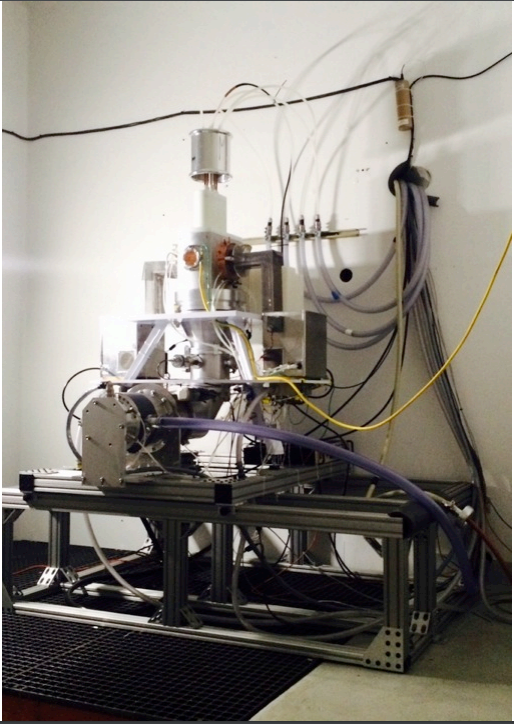
\includegraphics[width=\columnwidth]{./figures/Capture.PNG}
        \subfigimg[width=0.496\textwidth]{}{./figures/57Co_cum.pdf}{50}
%         \caption{ Decay curve for the $\beta^+$ decay of \ce{^{64}Cu}.}
%         \refstepcounter{subfigure} 
%         \label{fig:85gY}
   \hspace{-10pt}}%
    \\
    \subfloat{
        \centering
%         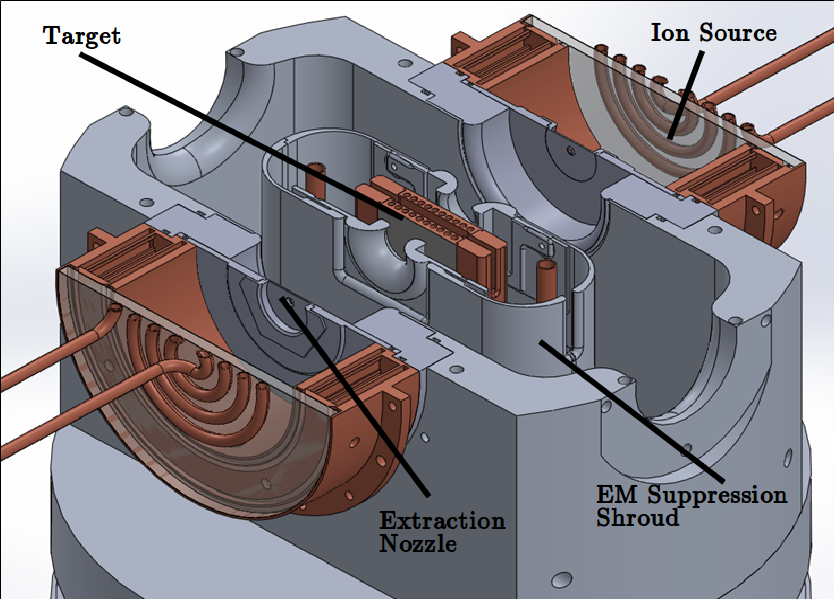
\includegraphics[width=\textwidth]{./figures/target2.png}
        \subfigimg[width=0.496\textwidth]{}{./figures/60Co.pdf}{50}
%         \caption{Decay curve for the $\beta^-$ decay of \ce{^{116}In}.}
        %         \refstepcounter{subfigure}
%          \label{fig:85mY}
%    }
%      \subfloat{
%         \centering
% %         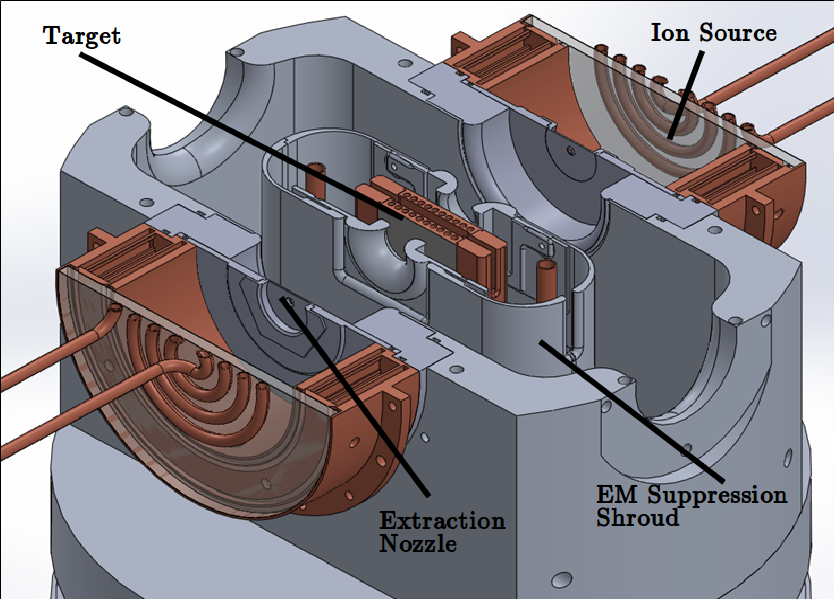
\includegraphics[width=\textwidth]{./figures/target2.png}
%         \subfigimg[width=0.496\textwidth]{}{./figures/86Y.pdf}{50}
% %         \caption{Decay curve for the $\beta^-$ decay of \ce{^{116}In}.}
%         %         \refstepcounter{subfigure}
%          \label{fig:86Y}
%    }
%     \\
%     \subfloat{
%         \centering
%         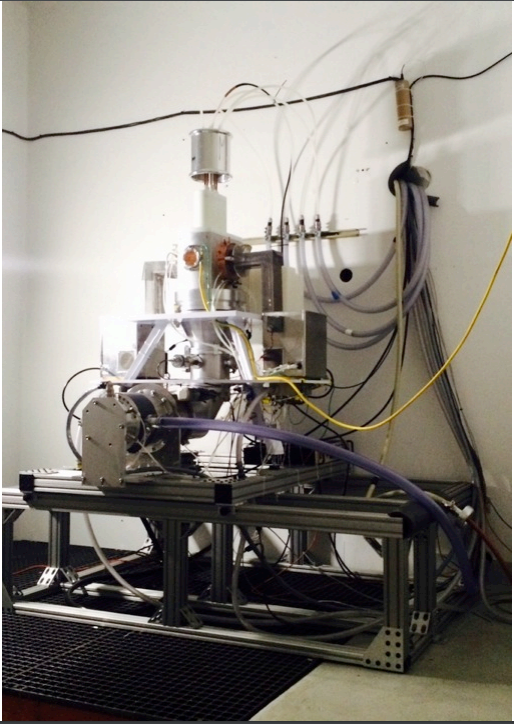
\includegraphics[width=\columnwidth]{./figures/Capture.PNG}
        \subfigimg[width=0.496\textwidth]{}{./figures/60Cu.pdf}{50}
%         \caption{ Decay curve for the $\beta^+$ decay of \ce{^{64}Cu}.}
%         \refstepcounter{subfigure}
%         \label{fig:86Zr}
   \hspace{-10pt}}%
    \\
    \subfloat{
        \centering
%         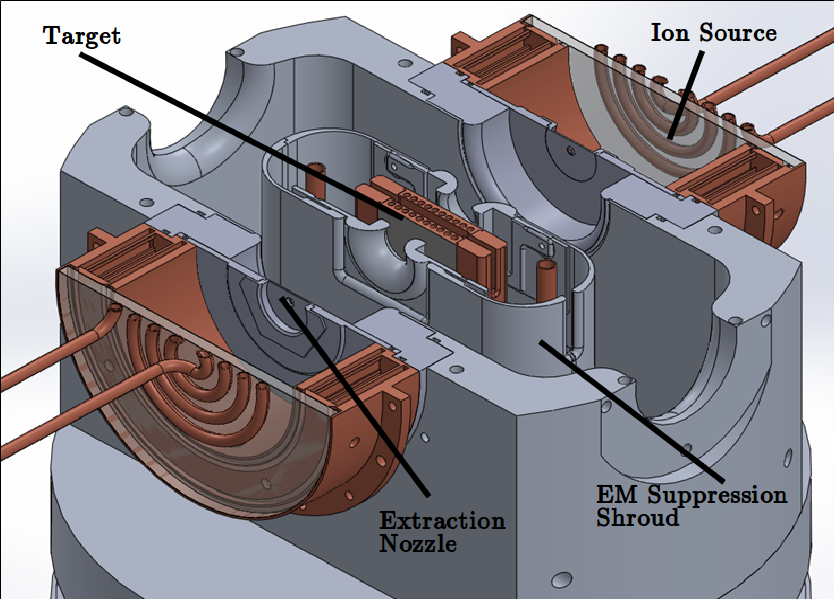
\includegraphics[width=\textwidth]{./figures/target2.png}
        \subfigimg[width=0.496\textwidth]{}{./figures/61Co.pdf}{50}
%         \caption{Decay curve for the $\beta^-$ decay of \ce{^{116}In}.}
        %         \refstepcounter{subfigure}
%          \label{fig:87Y}
%    }
%     \subfloat{
%         \centering
%         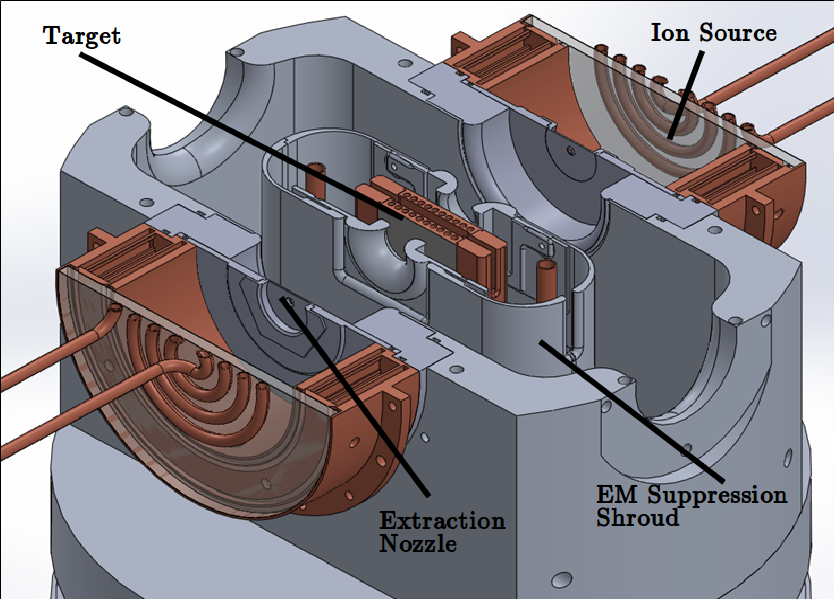
\includegraphics[width=\textwidth]{./figures/target2.png}
        \subfigimg[width=0.496\textwidth]{}{./figures/61Cu.pdf}{50}
%         \caption{Decay curve for the $\beta^-$ decay of \ce{^{116}In}.}
        %         \refstepcounter{subfigure}
%          \label{fig:87gY}
   \hspace{-10pt}}
%     \caption{Decay curves used to verify photopeak transition assignment. (a) Decay curve for the isomeric transition of \ce{^{115m}In}, (b) decay curve for the isomeric transition of \ce{^{113m}In}, (c) decay curve for the $\beta^-$ decay of \ce{^{116}In}, and (d) decay curve for the $\beta^+$ decay of \ce{^{64}Cu}.}
%      \phantomcaption{}\label{fig:xs_curves_p4}
\end{figure*}

\begin{figure*}
    \centering
     \subfloat{
        \centering
% %         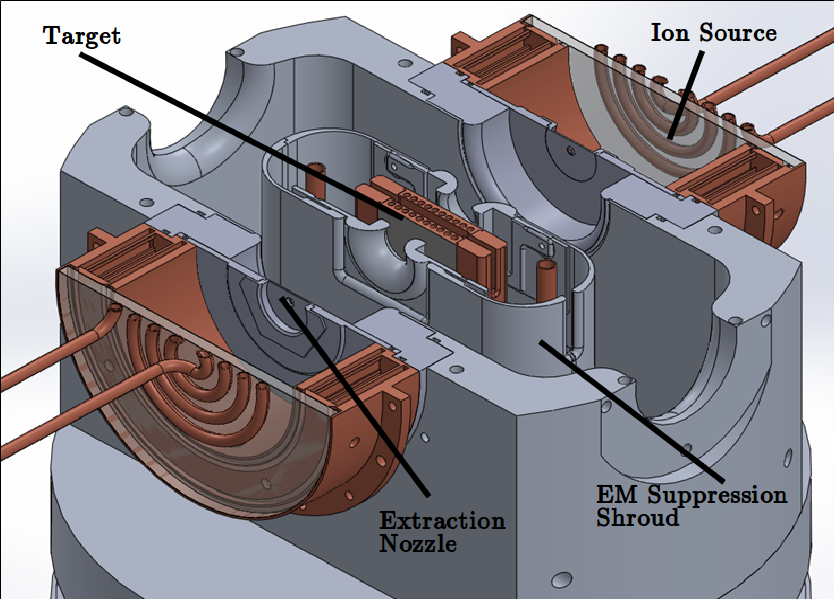
\includegraphics[width=\textwidth]{./figures/target2.png}
%         \subfigimg[width=0.496\textwidth]{}{./figures/87gY.pdf}{50}
% %         \caption{Decay curve for the $\beta^-$ decay of \ce{^{116}In}.}
%         %         \refstepcounter{subfigure}
%          \label{fig:87gY}
% %    }
%     \subfloat{
%         \centering
%         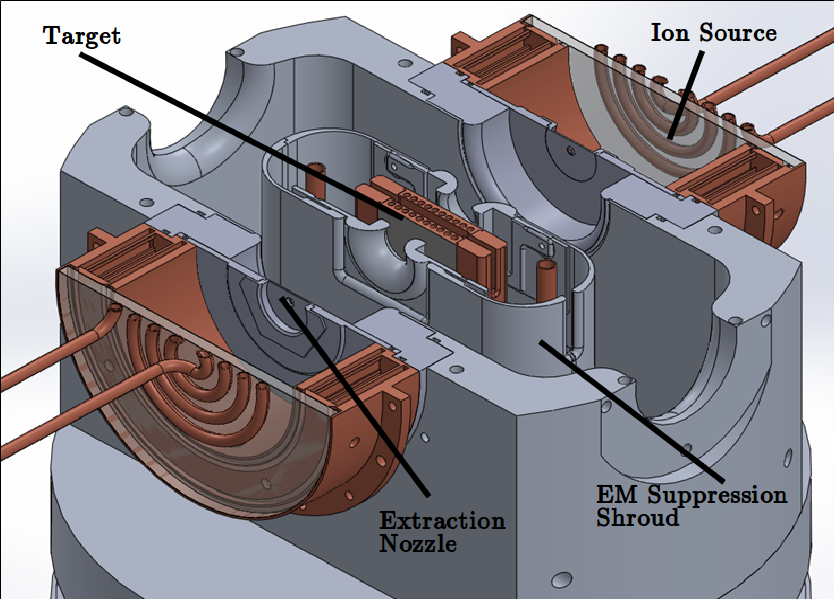
\includegraphics[width=\textwidth]{./figures/target2.png}
        \subfigimg[width=0.496\textwidth]{}{./figures/64Cu.pdf}{50}
%         \caption{Decay curve for the $\beta^-$ decay of \ce{^{116}In}.}
        %         \refstepcounter{subfigure}
%          \label{fig:87mY}
%    }
%     \subfloat{
%         \centering
%         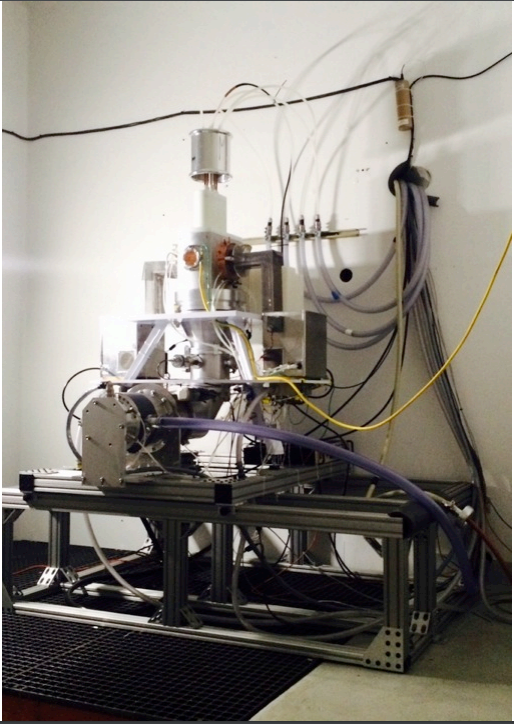
\includegraphics[width=\columnwidth]{./figures/Capture.PNG}
        \subfigimg[width=0.496\textwidth]{}{./figures/43K.pdf}{50}
%         \caption{ Decay curve for the $\beta^+$ decay of \ce{^{64}Cu}.}
%         \refstepcounter{subfigure}
%         \label{fig:87Zr}
   \hspace{-10pt}}%
    \\
    \subfloat{
        \centering
%         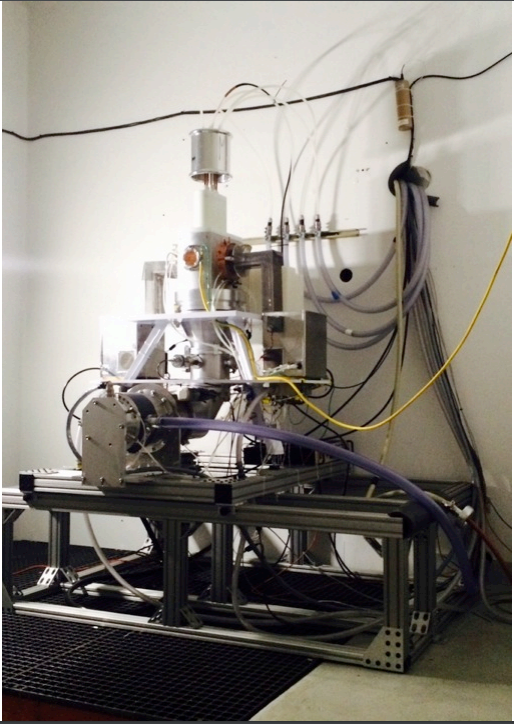
\includegraphics[width=\columnwidth]{./figures/Capture.PNG}
        \subfigimg[width=0.496\textwidth]{}{./figures/44mSc.pdf}{50}
%         \caption{ Decay curve for the isomeric transition of \ce{^{115m}In}.}
%         \refstepcounter{subfigure}
%          \label{fig:88Y}%
%         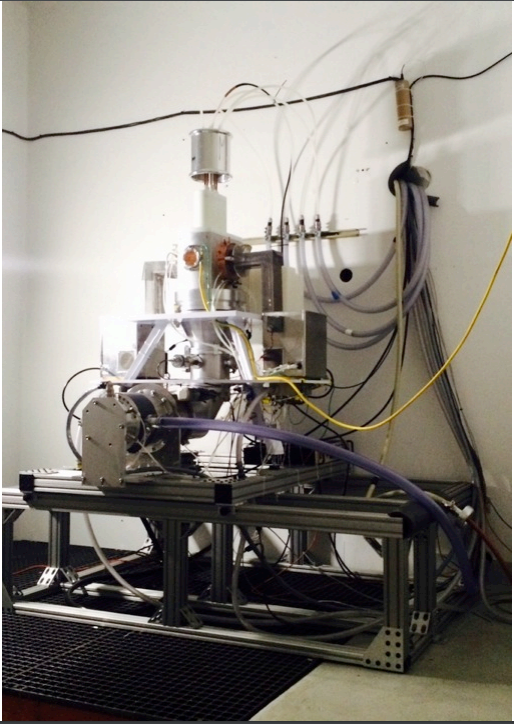
\includegraphics[width=\columnwidth]{./figures/Capture.PNG}
%         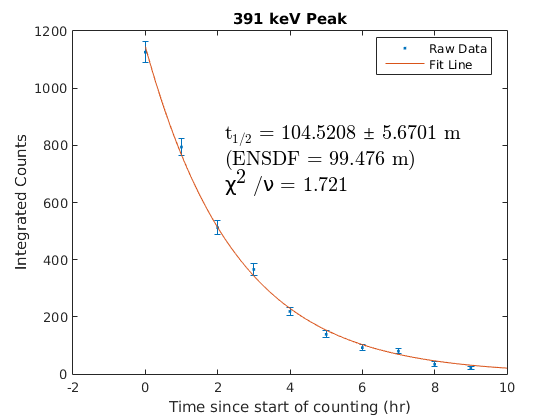
\includegraphics[scale=0.6]{./figures/391keV_curve2.png}
        \subfigimg[width=0.496\textwidth]{}{./figures/44gSc.pdf}{50}
%         \caption{ Decay curve for the isomeric transition of \ce{^{113m}In}.}
%         \refstepcounter{subfigure}
%          \label{fig:88Zr}
   \hspace{-10pt}}%
    \\
         \subfloat{
        \centering
%         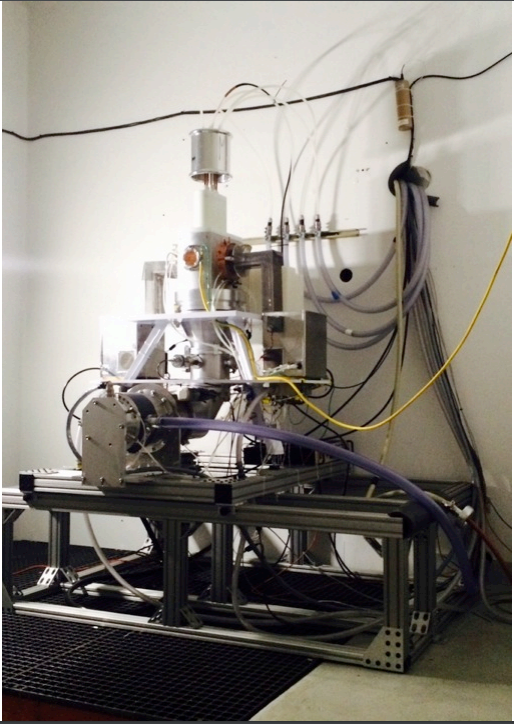
\includegraphics[width=\columnwidth]{./figures/Capture.PNG}
%         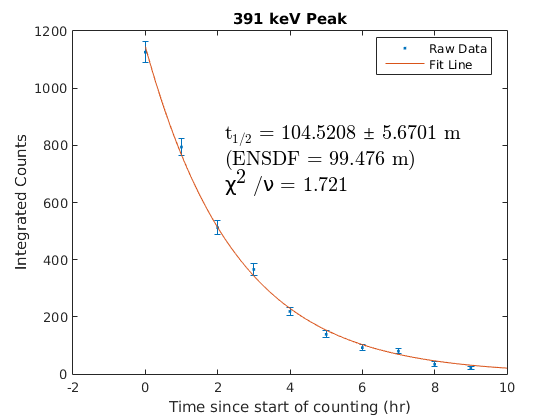
\includegraphics[scale=0.6]{./figures/391keV_curve2.png}
        \subfigimg[width=0.496\textwidth]{}{./figures/44Sc.pdf}{50}
%         \caption{ Decay curve for the isomeric transition of \ce{^{113m}In}.}
%         \refstepcounter{subfigure}
%          \label{fig:89Nb}
%    }%
%     \subfloat{
%         \centering
%         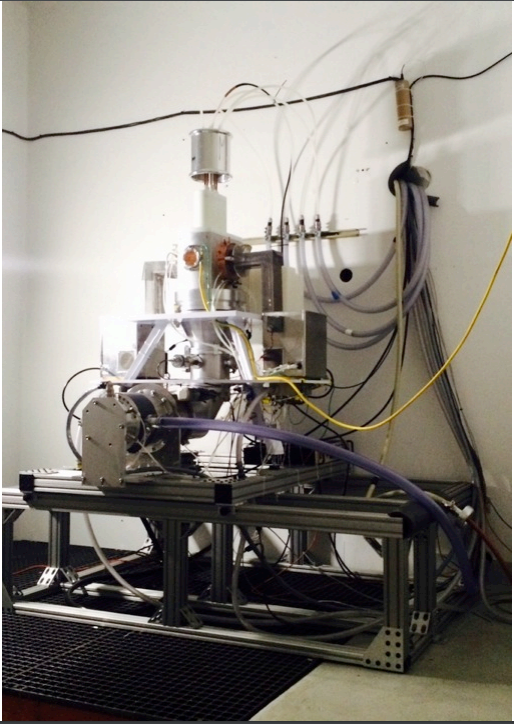
\includegraphics[width=\columnwidth]{./figures/Capture.PNG}
%         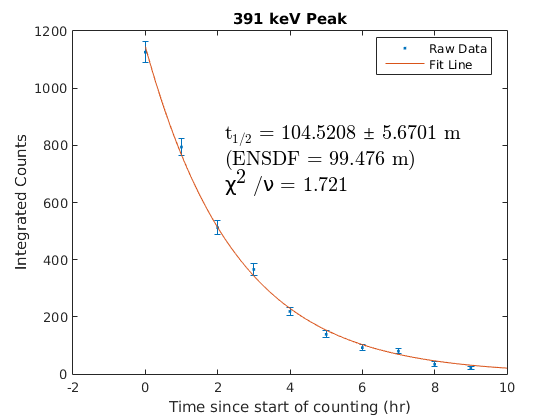
\includegraphics[scale=0.6]{./figures/391keV_curve2.png}
        \subfigimg[width=0.496\textwidth]{}{./figures/47Sc.pdf}{50}
%         \caption{ Decay curve for the isomeric transition of \ce{^{113m}In}.}
%         \refstepcounter{subfigure}
%          \label{fig:89gNb}
   \hspace{-10pt}}%
%     \caption{Decay curves used to verify photopeak transition assignment. (a) Decay curve for the isomeric transition of \ce{^{115m}In}, (b) decay curve for the isomeric transition of \ce{^{113m}In}, (c) decay curve for the $\beta^-$ decay of \ce{^{116}In}, and (d) decay curve for the $\beta^+$ decay of \ce{^{64}Cu}.}
%      \phantomcaption{}\label{fig:xs_curves_p8}
\end{figure*}
% 
\begin{figure*}
    \centering    
         \subfloat{
        \centering
% %         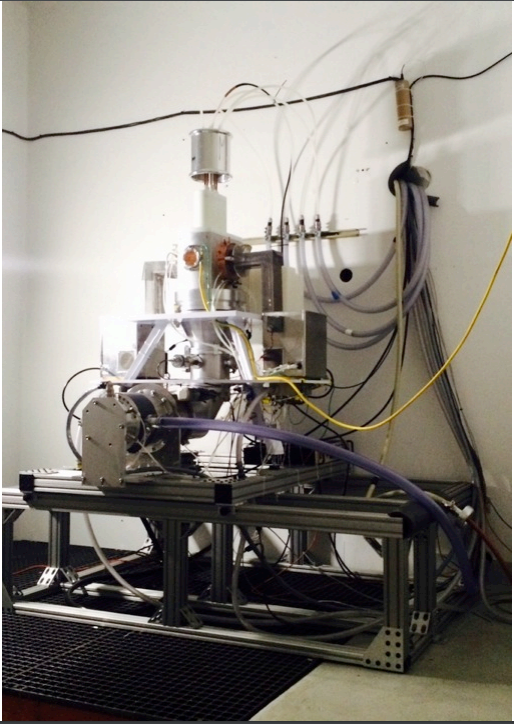
\includegraphics[width=\columnwidth]{./figures/Capture.PNG}
% %         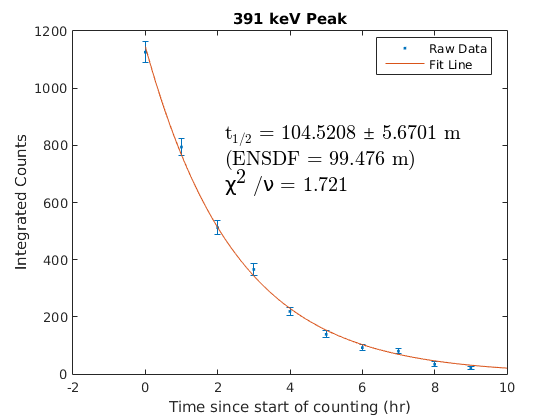
\includegraphics[scale=0.6]{./figures/391keV_curve2.png}
%         \subfigimg[width=0.497\textwidth]{}{./figures/89gNb.pdf}{50}
% %         \caption{ Decay curve for the isomeric transition of \ce{^{113m}In}.}
% %         \refstepcounter{subfigure}
%          \label{fig:89gNb}
% %    }%
%     \subfloat{
%         \centering
%         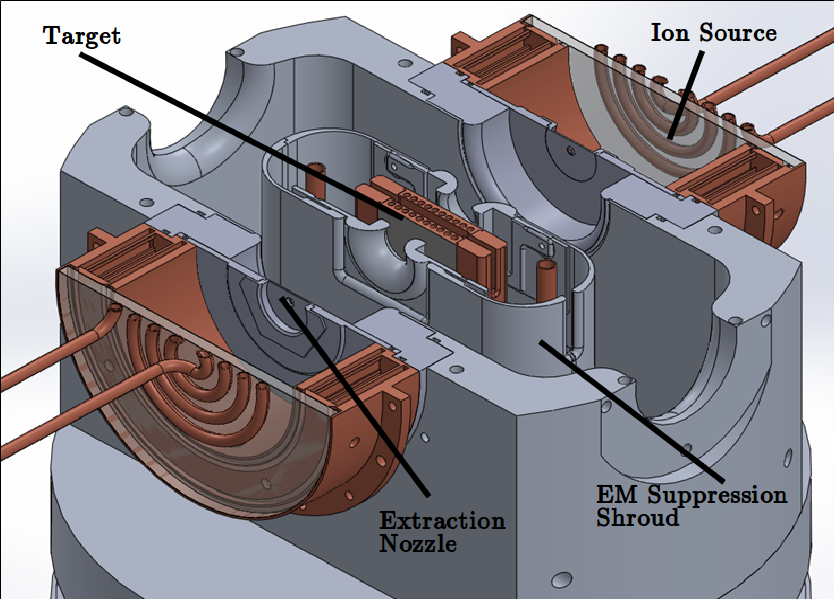
\includegraphics[width=\textwidth]{./figures/target2.png}
        \subfigimg[width=0.497\textwidth]{}{./figures/48Sc.pdf}{50}
%         \caption{Decay curve for the $\beta^-$ decay of \ce{^{116}In}.}
        %         \refstepcounter{subfigure}
%          \label{fig:89mNb}
% %    }
% %      \subfloat{
% %         \centering
% %         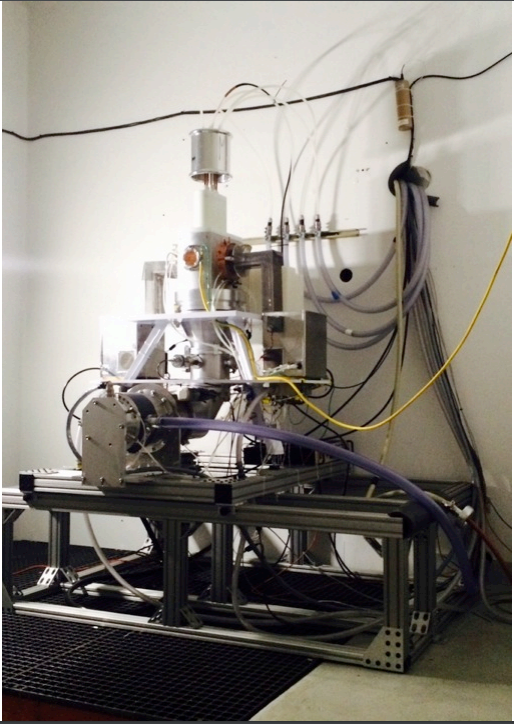
\includegraphics[width=\columnwidth]{./figures/Capture.PNG}
%         \subfigimg[width=0.497\textwidth]{}{./figures/89Zr.pdf}{50}
% %         \caption{ Decay curve for the $\beta^+$ decay of \ce{^{64}Cu}.}
% %         \refstepcounter{subfigure} 
% %         \label{fig:89Zr}
%    \hspace{-10pt}}%
%     \\
%     \subfloat{
%         \centering
% %         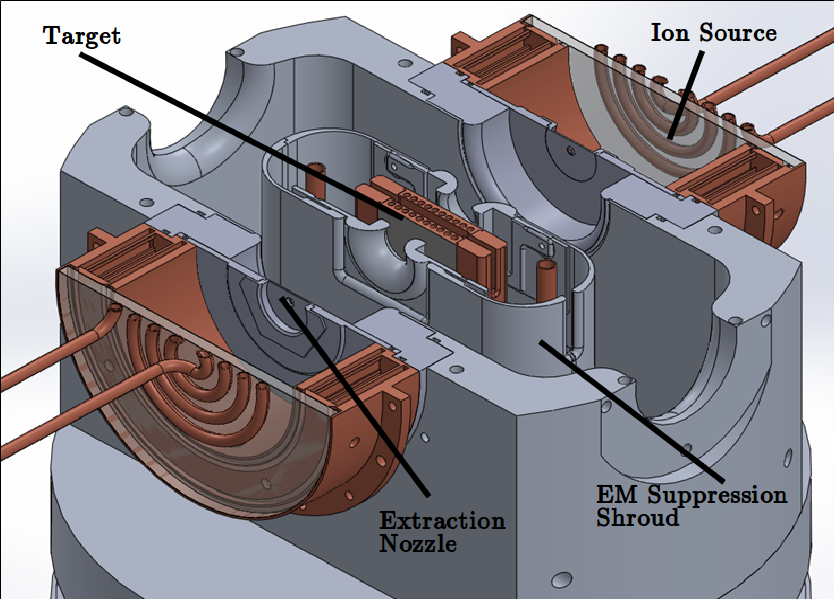
\includegraphics[width=\textwidth]{./figures/target2.png}
%         \subfigimg[width=0.497\textwidth]{}{./figures/91mNb.pdf}{50}
% %         \caption{Decay curve for the $\beta^-$ decay of \ce{^{116}In}.}
%         %         \refstepcounter{subfigure}
% %          \label{fig:91mNb}
% %    }
% %      \subfloat{
% %         \centering
% %         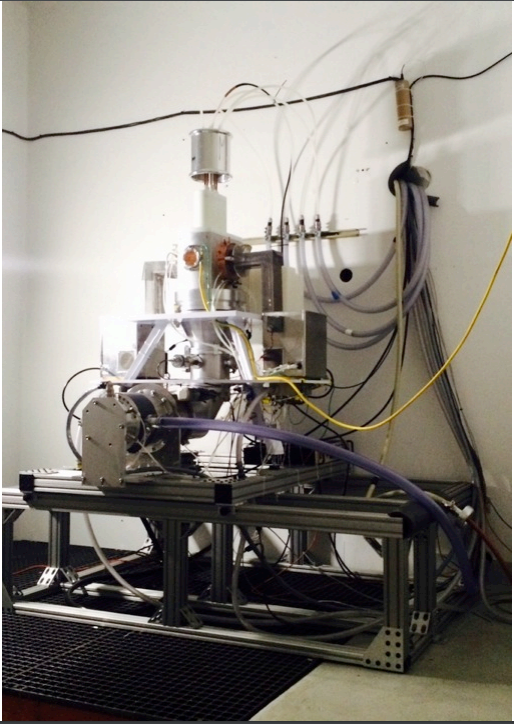
\includegraphics[width=\columnwidth]{./figures/Capture.PNG}
%         \subfigimg[width=0.497\textwidth]{}{./figures/92mNb.pdf}{50}
% %         \caption{ Decay curve for the $\beta^+$ decay of \ce{^{64}Cu}.}
% %         \refstepcounter{subfigure} 
% %         \label{fig:92mNb}
%    \hspace{-10pt}}%
%     \\
%     \subfloat{
%         \centering
% %         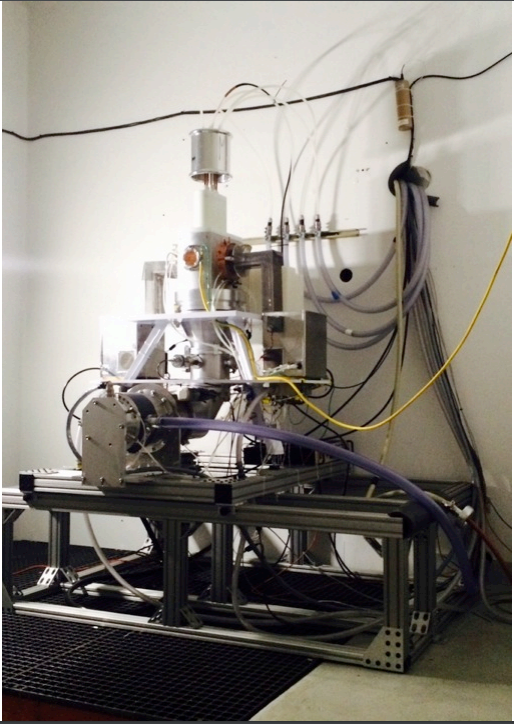
\includegraphics[width=\columnwidth]{./figures/Capture.PNG}
%         \subfigimg[width=0.497\textwidth]{}{./figures/93mMo.pdf}{50}
% %         \caption{ Decay curve for the isomeric transition of \ce{^{115m}In}.}
% %         \refstepcounter{subfigure}
% %          \label{fig:93mMo}
   }%
%     \caption{Decay curves used to verify photopeak transition assignment. (a) Decay curve for the isomeric transition of \ce{^{115m}In}, (b) decay curve for the isomeric transition of \ce{^{113m}In}, (c) decay curve for the $\beta^-$ decay of \ce{^{116}In}, and (d) decay curve for the $\beta^+$ decay of \ce{^{64}Cu}.}
%      \phantomcaption{}\label{fig:xs_curves_p7}
\end{figure*}
% 
% % \begin{figure*}
% %     \centering
% %     \subfloat{
% %         \centering
% % %         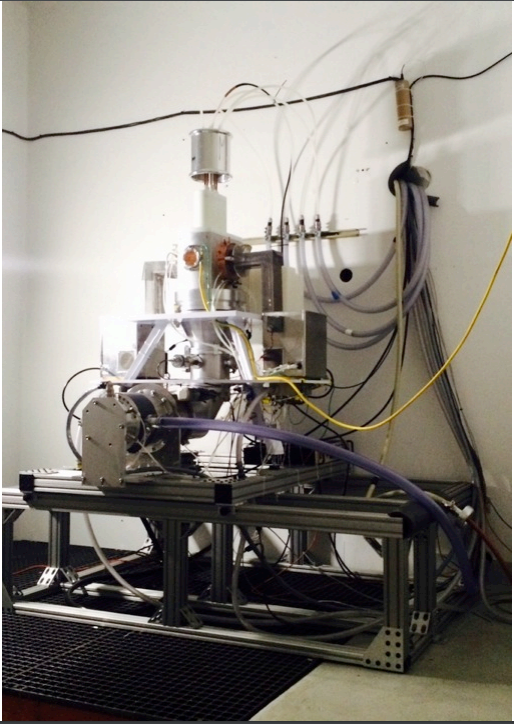
\includegraphics[width=\columnwidth]{./figures/Capture.PNG}
% %         \subfigimg[width=0.497\textwidth]{}{./figures/93mMo.pdf}{50}
% % %         \caption{ Decay curve for the isomeric transition of \ce{^{115m}In}.}
% % %         \refstepcounter{subfigure}
% %          \label{fig:93mMo}
% %    }%
% % %      \subfloat{
% % %         \centering
% % % %         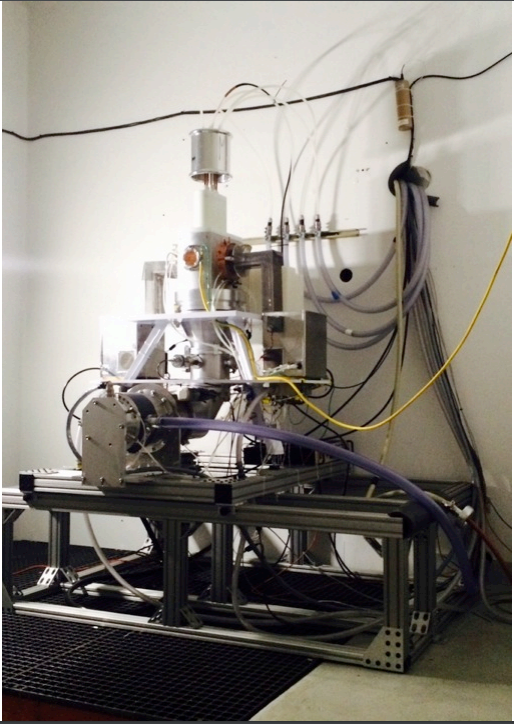
\includegraphics[width=\columnwidth]{./figures/Capture.PNG}
% % % %         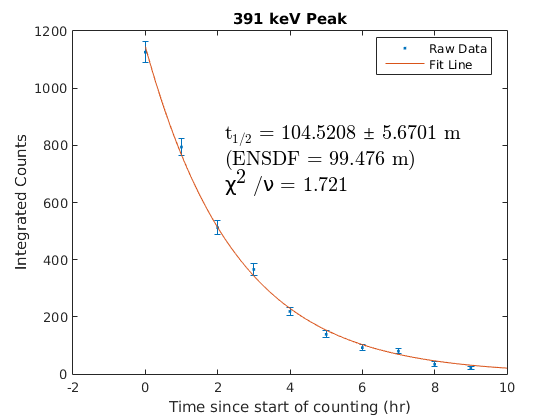
\includegraphics[scale=0.6]{./figures/391keV_curve2.png}
% % %         \subfigimg[width=0.497\textwidth]{}{./figures/91mNb.pdf}{50}
% % % %         \caption{ Decay curve for the isomeric transition of \ce{^{113m}In}.}
% % % %         \refstepcounter{subfigure}
% %          \label{fig:91mNb}
% % %    }%
% % %     \\
% % %     \subfloat{
% % %         \centering
% % % %         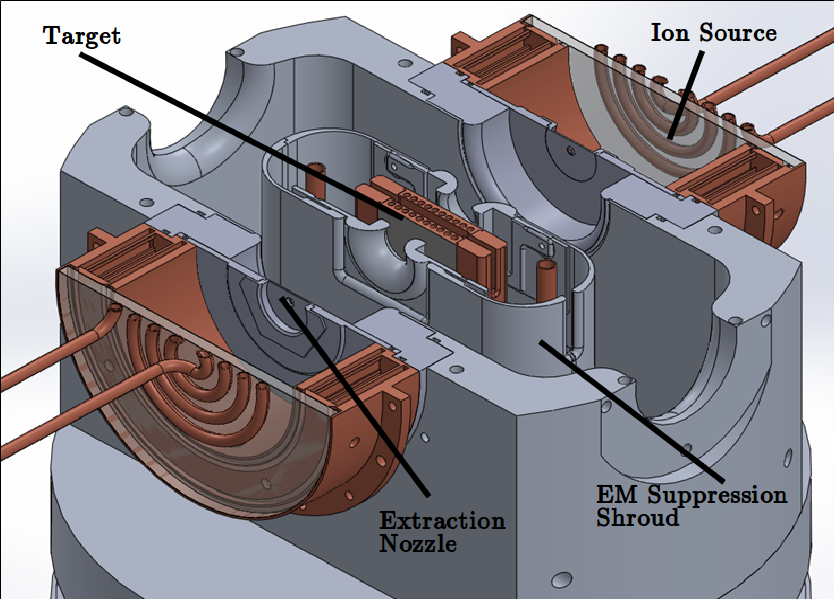
\includegraphics[width=\textwidth]{./figures/target2.png}
% % %         \subfigimg[width=0.497\textwidth]{}{./figures/92mNb.pdf}{50}
% % % %         \caption{Decay curve for the $\beta^-$ decay of \ce{^{116}In}.}
% % %         %         \refstepcounter{subfigure}
% %          \label{fig:92mNb}
% % %    }
% % %      \subfloat{
% % %         \centering
% % % %         \includegraphics[width=\columnwidth]{./figures/Capture.PNG}
% % %         \subfigimg[width=0.497\textwidth]{}{./figures/93mMo.pdf}{50}
% % % %         \caption{ Decay curve for the $\beta^+$ decay of \ce{^{64}Cu}.}
% % %%         \refstepcounter{subfigure} \label{fig:93mMo}
% % %    }%
% % %     \caption{Decay curves used to verify photopeak transition assignment. (a) Decay curve for the isomeric transition of \ce{^{115m}In}, (b) decay curve for the isomeric transition of \ce{^{113m}In}, (c) decay curve for the $\beta^-$ decay of \ce{^{116}In}, and (d) decay curve for the $\beta^+$ decay of \ce{^{64}Cu}.}
% %      \label{fig:xs_curves_p5}
% % \end{figure*}
% 
% 


% \pagebreak

% 
% 
\section{Measured isomer-to-ground state branching ratios } \label{sec:fe_ibr_figures}

Plots of the isomer-to-ground state ratios measured in this work are presented here, in comparison with literature data and reaction modeling codes 
\cite{Michel1978,Kopecky1993,Zarie2006a,Khandaker2009}.




     

\begin{figure*}
    \centering
    \subfloat{
        \centering
% %         \includegraphics[width=\columnwidth]{./figures/Capture.PNG}
        \subfigimg[width=0.497\textwidth]{}{./figures/52Mn_IBR.pdf}{50}
% %         \caption{ Decay curve for the isomeric transition of \ce{^{115m}In}.}
%         \refstepcounter{subfigure}
%          \label{fig:52Mn_IBR}%
%         \includegraphics[width=\columnwidth]{./figures/Capture.PNG}
%         \includegraphics[scale=0.6]{./figures/391keV_curve2.png}
        \subfigimg[width=0.497\textwidth]{}{./figures/58Co_IBR.pdf}{50}
%         \caption{ Decay curve for the isomeric transition of \ce{^{113m}In}.}
%         \refstepcounter{subfigure}
%          \label{fig:58Co_IBR}
   \hspace{-10pt}}%
    \\
    \subfloat{
        \centering
%         \includegraphics[width=\textwidth]{./figures/target2.png}
        \subfigimg[width=0.497\textwidth]{}{./figures/44Sc_IBR.pdf}{50}
%         \caption{Decay curve for the $\beta^-$ decay of \ce{^{116}In}.}
        %         \refstepcounter{subfigure}
%          \label{fig:85Y_IBR}
%    }
% %      \subfloat{
% %         \centering
% %         \includegraphics[width=\columnwidth]{./figures/Capture.PNG}
%         \subfigimg[width=0.497\textwidth]{}{./figures/87Y_IBR.pdf}{50}
% %         \caption{ Decay curve for the $\beta^+$ decay of \ce{^{64}Cu}.}
% %         \refstepcounter{subfigure} 
% %         \label{fig:87Y_IBR}
%    \hspace{-10pt}}%
%     \\
%     \subfloat{
%         \centering
% %         \includegraphics[width=\textwidth]{./figures/target2.png}
%         \subfigimg[width=0.497\textwidth]{}{./figures/89Nb_IBR.pdf}{50}
% %         \caption{Decay curve for the $\beta^-$ decay of \ce{^{116}In}.}
%         %         \refstepcounter{subfigure}
% %          \label{fig:89Nb_IBR}
   }
%      \phantomcaption{}\label{fig:ibr_curves}
\end{figure*}


\pagebreak


% 
% 
\section{Stack design } \label{sec:fe_stack_design}

% Plots of the isomer-to-ground state ratios measured in this work are presented here, in comparison with literature data and reaction modeling codes 
% \cite{Michel1978,Kopecky1993,Zarie2006a,Khandaker2009}.





% Combined table
% Please add the following required packages to your document preamble:
% \usepackage{booktabs}
\begin{table*}[h!]
\centering
\caption{Specifications of the 25\,MeV and 55\,MeV target stack designs in the present work. The proton beam enters the stack upstream of the SS-5 and SS-3 profile monitors, respectively, and travels through the stack in the order presented here. The 6061 aluminum degraders have a measured density of approximately 2.68 $\pm$ 0.03 g/cm$^3$. Their areal densities were determined using the variance minimization techniques described  in this work  and an earlier paper\,\cite{Voyles2018a}. 
% the earlier paper by Graves \etal\\,\cite{Graves2016}.
A 316 stainless steel foil is inserted at both the front and rear of each target stack as a monitor of the beam's spatial profile, by developing radiochromic film (Gafchromic EBT3) after end-of-bombardment (EoB).}
\label{tab:fe_stack_table}
\small
\resizebox{\textwidth}{!}{%
\begin{tabular}{@{}llll|llll@{}}
\toprule\toprule
% Target Layer       & Nominal Thickness & Measured thickness (mg/cm\textasciicircum 2) & Thickness Uncertainty (\%) \\ \midrule
25\,MeV Target layer            & \begin{tabular}[c]{@{}l@{}}Measured \\ thickness\end{tabular} & \begin{tabular}[c]{@{}l@{}}Measured\\areal density\\(mg/cm$^2$)\end{tabular} & \begin{tabular}[c]{@{}l@{}}Uncertainty \\ in areal\\ density  (\%)\end{tabular} & 55\,MeV Target layer            & \begin{tabular}[c]{@{}l@{}}Measured \\ thickness\end{tabular} & \begin{tabular}[c]{@{}l@{}}Measured\\areal density\\(mg/cm$^2$)\end{tabular} & \begin{tabular}[c]{@{}l@{}}Uncertainty \\ in areal\\ density  (\%)\end{tabular} \\
\midrule
SS profile monitor SS-5 & 130.94 \mmicro m                                              & 100.57                                                                      & 0.17                                                                      & SS profile monitor SS-3 & 130.9 \mmicro m                                               & 100.48                                                                      & 0.17                                                                      \\
Fe-08                   & 26.25 \mmicro m                                               & 19.69                                                                       & 0.17                                                                      & Fe-01                   & 25.75 \mmicro m                                               & 20.22                                                                       & 0.21                                                                      \\
Ti-14                   & 25.01 \mmicro m                                               & 10.87                                                                       & 0.36                                                                      & Ti-01                   & 25.88 \mmicro m                                               & 11.09                                                                       & 0.16                                                                      \\
Cu-14                   & 24.01 \mmicro m                                               & 17.49                                                                       & 0.40                                                                      & Cu-01                   & 28.81 \mmicro m                                               & 22.40                                                                       & 0.11                                                                      \\
Al Degrader E-09        & 256.5 \mmicro m                                               & --                                                                          & --                                                                        & Al Degrader A-1         & 2.24 mm                                                       & --                                                                          & --                                                                        \\
Fe-09                   & 26.5 \mmicro m                                                & 19.90                                                                       & 0.09                                                                      & Fe-02                   & 25.5 \mmicro m                                                & 19.91                                                                       & 0.13                                                                      \\
Ti-15                   & 23.81 \mmicro m                                               & 10.97                                                                       & 0.11                                                                      & Ti-02                   & 25.74 \mmicro m                                               & 10.94                                                                       & 0.24                                                                      \\
Cu-15                   & 21.81 \mmicro m                                               & 17.63                                                                       & 0.46                                                                      & Cu-02                   & 28.75 \mmicro m                                               & 22.32                                                                       & 0.40                                                                      \\
Al Degrader H-01        & 127.09 \mmicro m                                              & --                                                                          & --                                                                        & Al Degrader A-2         & 2.24 mm                                                       & --                                                                          & --                                                                        \\
Fe-10                   & 26.5 \mmicro m                                                & 19.84                                                                       & 0.11                                                                      & Fe-03                   & 25.25 \mmicro m                                               & 20.00                                                                       & 0.27                                                                      \\
Ti-16                   & 24.6 \mmicro m                                                & 10.96                                                                       & 0.32                                                                      & Ti-03                   & 25.91 \mmicro m                                               & 11.25                                                                       & 0.15                                                                      \\
Cu-16                   & 22.01 \mmicro m                                               & 17.22                                                                       & 0.25                                                                      & Cu-03                   & 28.86 \mmicro m                                               & 22.49                                                                       & 0.20                                                                      \\
Fe-11                   & 27.26 \mmicro m                                               & 19.96                                                                       & 0.17                                                                      & Al Degrader C-1         & 0.97 mm                                                       & --                                                                          & --                                                                        \\
Ti-17                   & 25.01 \mmicro m                                               & 10.88                                                                       & 0.25                                                                      & Fe-04                   & 25.25 \mmicro m                                               & 19.93                                                                       & 0.33                                                                      \\
Cu-17                   & 29 \mmicro m                                                  & 21.91                                                                       & 0.33                                                                      & Ti-04                   & 25.84 \mmicro m                                               & 10.91                                                                       & 0.18                                                                      \\
Fe-12                   & 27.01 \mmicro m                                               & 20.03                                                                       & 0.12                                                                      & Cu-04                   & 28.78 \mmicro m                                               & 22.38                                                                       & 0.29                                                                      \\
Ti-18                   & 25.01 \mmicro m                                               & 11.00                                                                       & 0.87                                                                      & Al Degrader C-2         & 0.97 mm                                                       & --                                                                          & --                                                                        \\
Cu-18                   & 28.75 \mmicro m                                               & 22.33                                                                       & 0.14                                                                      & Fe-05                   & 25.64 \mmicro m                                               & 20.02                                                                       & 0.24                                                                      \\
Fe-13                  & 26.25 \mmicro m                                               & 20.05                                                                       & 0.16                                                                      & Ti-05                   & 25.86 \mmicro m                                               & 10.99                                                                       & 0.30                                                                      \\
Ti-19                   & 26.6 \mmicro m                                                & 11.01                                                                       & 0.22                                                                      & Cu-05                   & 28.77 \mmicro m                                               & 22.35                                                                       & 0.12                                                                      \\
Cu-19                   & 28.75 \mmicro m                                               & 22.32                                                                       & 0.19                                                                      & Al Degrader C-3         & 0.97 mm                                                       & --                                                                          & --                                                                        \\
Fe-14                   & 25.75 \mmicro m                                               & 20.11                                                                       & 0.19                                                                      & Fe-06                   & 25.75 \mmicro m                                               & 20.21                                                                       & 0.26                                                                      \\
Ti-20                   & 27.01 \mmicro m                                               & 11.06                                                                       & 0.35                                                                      & Ti-06                   & 25.5 \mmicro m                                                & 11.15                                                                       & 0.23                                                                      \\
Cu-20                   & 28.26 \mmicro m                                               & 22.34                                                                       & 0.28                                                                      & Cu-06                   & 28.83 \mmicro m                                               & 22.43                                                                       & 0.10                                                                      \\
SS profile monitor SS-6 & 131.5 \mmicro m                                               & 100.99                                                                      & 0.17                                                                      & Al Degrader C-4         & 0.97 mm                                                       & --                                                                          & --                                                                        \\
                        &                                                               &                                                                             &                                                                           & Fe-07                   & 25.76 \mmicro m                                               & 19.93                                                                       & 0.19                                                                      \\
                        &                                                               &                                                                             &                                                                           & Ti-07                   & 25.75 \mmicro m                                               & 11.17                                                                       & 0.33                                                                      \\
                        &                                                               &                                                                             &                                                                           & Cu-07                   & 28.76 \mmicro m                                               & 22.34                                                                       & 0.24                                                                      \\
                        &                                                               &                                                                             &                                                                           & Al Degrader H-02        & 127.04 \mmicro m                                              & --\cmmnt{34.51}                                                                       & --\cmmnt{0.20}                                                                      \\
                        &                                                               &                                                                             &                                                                           & SS profile monitor SS-4 & 131.21 \mmicro m                                              & 101.25                                                                      & 0.16                                                                     \\
 \bottomrule\bottomrule
\end{tabular}
}
\end{table*}
